\section{Few Shot Learning}
%What to expect
This section will explain what \textit{Few Shot Learning (FSL)} is, and why FSL has seen a considerable amount of interest. Furthermore, it will present relevant terminology and different approaches to solving the problem of FSL.

%Motivation + general overview
Conventional machine learning models have been shown to be highly accurate at classification and regression. However, the problem is that these models require immense datasets to be effective, and as a result the smaller the dataset the worse the result. FSL tries to solve the problem of being accurate on small datasets by using prior knowledge, which makes it able to generalise on new tasks on only a few data samples \cite{fsl2019}.

%Introduction to FSL
Humans are capable of quickly applying previously learned information to a new task, e.g. a child that has never seen the number "1" \textit{Query} before, is able to classify what class it belongs by only using other numbers \textit{(Support Set)}. This is illustrated in the \ref{fig:query_support}, where the child is given a picture of the number "1", and a support set of five other numbers which include the query class. The child is able to successfully identify which of the five classes is the same as the query class by using his prior knowledge. The number of classes in the support set is known as N-way, and the number of samples of each class is the K-shot. This is typically known as N-way-K-Shot classification. As one can imagine from the given example, the more K-shots the child has the easier it might be to classify, and the larger the N-way, the harder it is, since some classes might share similarities which could result in a wrong classification. Additionally, if one has to predict a query class and has support sets $|S_1| = 5$ and $|S_2| = 10$, and one picks a random class the probability of a correct guess is respectively, $20\%$ and $10\%$. Hereafter, we will introduce FSL in a more formal manner.

%Formal introduction 
Moreover, given a learning task $\mathcal{T}$ and a dataset $\mathcal{D}=\{\mathcal{D}_{train}, \mathcal{D}_{test}\}$. The training set is defined as $\mathcal{D}_{train} = \{{(x_i, y_i)}\}^{I}_{i=1}$, where I is very small compoared to traditional datasets. The test set is defined as $\mathcal{D}_{test}=\{x^{test}\}$
 

\begin{figure}
    \centering
    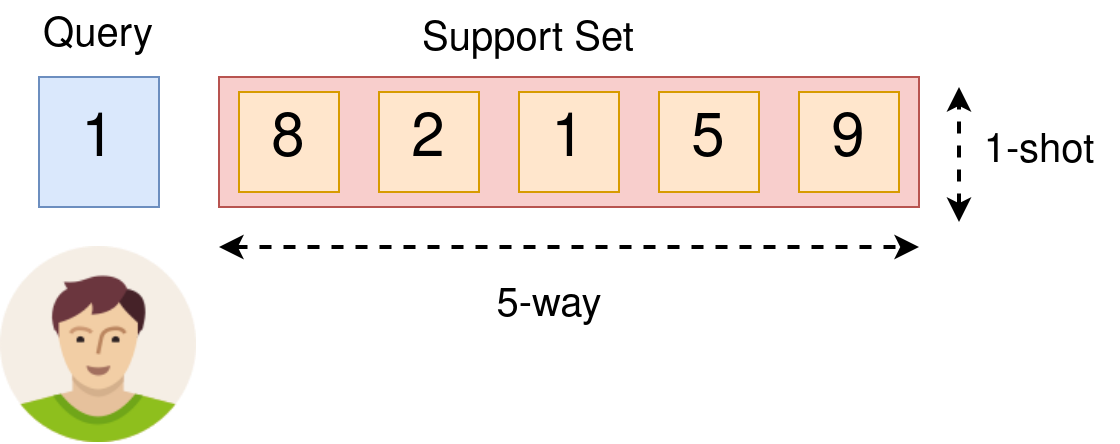
\includegraphics[scale=0.25]{img/prerequisites/query_support.png}
    \caption{Few shot learning example}
    \label{fig:query_support}
\end{figure}



\subsubsection{Protonets}

